\newtheorem{theorem}{Theorem}
\ifx \definition \undefined
	\newtheorem{definition}{Definition}
\fi	
\newtheorem{lemma}{Lemma}
\newtheorem{assumption}{Assumption}

\chapter{Virtual Modular Diagnosability}
\label{chap:theory}

This chapter presents the virtual modular diagnosability, a new type of
diagnosability. After a formal definition of the notion, it proceeds with an
analysis of a simple system which consists of two modules, modeled by automata.
This analysis exposes structural conditions for the models, such that
a verification whether the models satisfy these conditions allows to infer
diagnosability property of their composition, i.e of the entire system. Then
these conditions are rewritten for a general case, i.e. a system that consists
of an arbitrary number of components. The chapter then presents algorithms which
facilitate diagnosability verification in a efficient way. At the end, a
simple abstract example shows application of this approach.  

The final goal is to make a given system modularly diagnosable. Lets assume
that the system is diagnosable globally with respect to a given fault. It
implies that it is always possible to find a subset of the system's modules,
such that it contains a faulty module, and all the modules from the subset can
be composed into one locally diagnosable module. Each module in the subset helps
to detect and distinguish the fault by sequences of its observable events. The
assumption also implies that not each module of the system can or may
participate in the fault detection and distinguishing process. 

\section{Formal Definition}

Mathematically speaking, if the initial modularity does not satisfy the property
of modular diagnosability, then we need to find a partition of the set of the
modules such that all the modules in each element of the partition can be
considered as a \emph{virtual module}, and the system with the new modularity
satisfies the property of modular diagnosability.

The setup for the problem is following. Let a system be defined as a set of
local languages $\{L_{i\in I}\}$, and let a faulty behaviour be defined for any
$i \in I$, i.e. each language $L_i$ can be disjoint into faulty and non-faulty
sublanguages: $L_{i,f}$ and $L_{i,nf}$. 
% We assume that a faulty behaviour is
% defined in a \emph{specification-based}, rather then \emph{event-based}, way.
For the sake of simplicity, we assume that a language may have only one type of
fault. We assume that $(\forall i \in I)\left[ L_i = P_i(L)\right]$. The
motivation for this assumption is following. Most of real-life complex systems
are of high modularity, where each module is presented as a small model along
with corresponding faults as, for example, in \cite{sartini_methodology_2010}.
When properly designed, such systems have neither deadlocks nor trajectories
which never executed. In practice, such assumption may require construction of a
supervisor, and verification that a local language of each module is globally
consistent, before checking diagnosability of the system.

\begin{definition}
Let $J$ be a partition of $I$. Given a set of system's languages $\{L_{i \in
I}\}$ and a set of observable projections $\{M_j \mid j \in J \}$. 
The system is modularly diagnosable with respect to $J$ and $\{M_j\}$ 
if the following holds:
\end{definition}
\begin{equation}
	\begin{array}{l}
		\forall(i \in I, s \in L_{i,f}, t \in L_{i,f}/s)
		\\
		(\exists n \in \mathbb{N})
		(|t| \geq n)
		\\
		\left[ M_j(P_i^{-1}(st)) \cap M_j(P_i^{-1}(L_{i,nf})) = \emptyset \right].
	\end{array}
\end{equation}
The definition requires each fault originated in any language of the subset $j$
to be diagnosed by observing only events of the languages from the same subset
$j$.

A trivial solution for the above problem is to enumerate all the partitions of
the set and check whether the result of composition of each element of the
partition is locally diagnosable. In general, the total number of partitions of
a set with cardinality $n$ is known as the Bell number $B_n$, which has a double
exponential generation function \cite{brualdi_introductory_2004}.

In reality, it may not necessary to enumerate all the partitions, since a
partition which corresponds to modularly diagnosable system can be found even at
the first iteration. Moreover, it is not necessary to compose all the modules of
each element of the partitions, since not all partition's elements may contain
modules with faults. However, the level of complexity in the worst case
motivates us to find a more smart solution for the problem.

In the next section we make the first step toward a feasible approach for the
problem.


\section{Trivial system. Analysis of two adjacent modules}

As was mentioned above, the first step to improve the search for a relevant
partition, is to enumerate only the modules which potentially can influence
diagnosability. Firstly, those are ones which have observable events. Then, the
structure of modules may have some patterns, such that if a pattern is found,
then we can infer its influence before the module is composed with others.
The module with the fault may also be analyzed for a possibility to change its
observation due to interaction with other modules. Thus, in the trivial case of
a system consisting of two modules where only one module has a fault, in order
to solve the problem, we need to answer the following questions: a) can a
module with a fault potentially change observations of its strings while
composed with the adjacent module? and b) can a module change observation of
some strings of another module due to concurrency? No parallel composition should be
used in order to answer the questions. Otherwise, the problem would reduce to
the problem of local diagnosability.

We suppose that the system consists only of two modules with the corresponding
languages $L_1$ and $L_2$. The language of the system is $L := L_1 \parallel
L_2$. Suppose that only one module has a faulty behaviour: $L_1 := L_{1,f}
~\dot{\cup}~ L_{1,nf}$.
Suppose that $L_1$ is not diagnosable locally, but $L$ is diagnosable.

Firstly, we define the notion of observation changing of a string in a global
language.
\begin{definition}Given two languages $L_1$ and $L_2$. A string $s \in
L_1$ \emph{changes its observation} $M_1(s)$ in the language $L$ if
there is no the same observation in $P_1^{-1}(s)$, i.e.
if the following holds:
\end{definition}
\begin{equation}
\label{def:obs}
	\begin{array}{l}
		M(L) \cap M_1(s) = \emptyset.
	\end{array}
\end{equation}

\begin{lemma}
\label{lem_changed_observation}
Given two languages $L_1$ and $L_2$, and a string $s \in L_1$.
Assume that $s \in P_1(L)$. The string $s$ changes its observation in the
language $L$ if and only if:
\end{lemma}
\begin{subequations}\label{lem:obs}
\begin{align}
	(\exists \sigma \in s \mid \sigma \in \Sigma_1 \cap \Sigma_2) \land
	\label{lem:obs1}
	\\
	(\forall t\sigma \in L_2)
	\left[M_2(t) \neq \emptyset \right],
	\label{lem:obs2}
	\\
	\textrm{where } M_2: \Sigma^* \rightarrow (\Sigma_{2,o} \backslash
	\Sigma_1)^*. 
	\label{lem:obs3}
\end{align}
\end{subequations}

\begin{proof}
In order to prove sufficiency of (\ref{lem:obs}) we use its converse relation
and prove by contradiction that the change of observation (\ref{def:obs}) is
necessary.
Assume it $\exists w \in L$ and $\exists s \in L_1$ such that
$M(w)= M_1(s)$ and, therefor, (\ref{def:obs}) is false. Let $\exists
\sigma \in \Sigma_1 \cap \Sigma_2$ such that $\sigma \in w$ and also
(\ref{lem:obs1}) holds. Then may $\exists u \sigma \in \overline{w}$ such that
$M_2(u) = \emptyset$, and then $M_2(P_2(u)) =
\emptyset$ which contradicts (\ref{lem:obs2}). Now, let (\ref{lem:obs2})
be true for all $t\sigma \in P_2(w)$. Then the assumption $M(w)=
M_1(s)$ holds only if $\sigma \not \in s$, which contradicts (\ref{lem:obs1}). 

We prove necessity of (\ref{lem:obs}) by contradiction.
Let (\ref{lem:obs1}) holds, and $\exists t\sigma \in L_2$ such that
$M_2(t) = \emptyset$. Then may $\exists t'\sigma \in 
L \subseteq P_2^{-1}(t\sigma)$ such that $M_2(t') =
\emptyset$ and $M_1(t') = M_1(s) \neq \emptyset$, which contradicts
(\ref{def:obs}).
Now, let (\ref{lem:obs2}) holds and $\not \exists \sigma \in s' \in P_1^{-1}(s)
\mid \sigma \in \Sigma_1 \cap \Sigma_2$. Then may $\exists w \in L_2$ and,
hence, $w' \in L \subseteq P_2^{-1}(w)$ such that $M(w')=M(s)$,
which contradicts (\ref{def:obs}).
\end{proof}

Informally, the above lemma says that the string of the local language $L_1$
changes its observation in the global language $L$ if and only if the string has
an event in common with the language $L_2$, and all the strings of $L_2$ which
have this common event have observable events in the prefixes, and some of the
observable events in the prefixes are not common with $L_1$.

We call the subset of stings $\{t \in L_2\}$ satisfying condition
(\ref{lem:obs2}) as the \emph{adjacent observable support} for the given string
$s \in L_1$.

\begin{definition} Given two languages $L_1$ and $L_2$. We say that a string $s
\in L_{1}$ is distinguished from all the other local strings $L_1\backslash s$
in the language $L$ if the following holds:
\end{definition}
\begin{equation}
\label{def:dist}
\begin{array}{l}
% 		M(s \parallel L_2) \cap M((L_1\backslash s) \parallel L_2)
% 		= \emptyset.
  (\forall w \in L_1\backslash s)\\
  	\left[ MP_1^{-1}(w \parallel L_2) \cap MP_1^{-1}(s\parallel L_2) = \emptyset
  	\right].
\end{array}
\end{equation}

\begin{lemma}
\label{lem:distinguished_for_2}
Given two languages $L_1$ and $L_2$. Assume that $L_1 = P_1(L)$. The string $s
\in L_1$ is distinguished from $L_1\backslash s$ in the language $L$ if $s$ has
an adjacent observable support $L_{2,s} \subseteq L_2$ which
satisfies the following condition:
\end{lemma}
\begin{subequations}
\begin{align}
	(\forall t \in L_{2,s})
	\left[ \exists \sigma \in t \mid \sigma \in \Sigma_1 \cap \Sigma_2)\right]
	\land
	\label{lem:dist1}
	\\
	(\forall w \in L_1\backslash s)\left[\sigma \not \in w \right]
	\label{lem:dist2} \land
	\\
	(\forall t'\sigma \in \overline{t})
	[M_2(t / t'\sigma) \neq \emptyset]
	\label{lem:dist3},
\end{align}
\end{subequations}

where $M_2$ is defined as in (\ref{lem:obs3}). 

\begin{proof}
Assume (\ref{def:dist}) is false, i.e. $\exists w' \in P_1^{-1}(w)$ and $\exists
s' \in P_1^{-1}(s)$ such that $M(w') = M(s')$. 

Assume (\ref{lem:dist1}) and (\ref{lem:dist2}) hold. Then may $\exists t' \in
\overline{s'} \mid t' \in P_2^{-1}(L_{2,s})$ such that $M(t') = M(w')$, and $t
\in P_2(t')$ such that $M_2(t) = M_2(w)$. And may $\exists t'' \in \overline{t}$
such that $M_2(t'') = M_2(w)$. Since $\sigma \in t$ and $\sigma \not \in w$,
then $M(t \backslash t''\sigma) = \emptyset$ for any $t''\sigma \in
\overline{t}$, which contradicts (\ref{lem:dist3}).

Assume (\ref{lem:dist1}) and (\ref{lem:dist3}) hold. Let $M_1(L_1) = \emptyset$
and $M_2(t\backslash t'\sigma) = M_2(s) = M_2(s)$. Then $\forall s' \in
M(P_1^{-1}(s))$ there exists $\sigma \in s'$, which contradicts
(\ref{lem:dist2}).

Assume (\ref{lem:dist2}) and (\ref{lem:dist3}) hold. If (\ref{def:dist}) is
false, then (\ref{lem:dist1}) is false. However, (\ref{lem:dist3}) is sufficient
for (\ref{lem:dist1}), which contradicts the former statement.
\end{proof}

Informally, the above lemma says that a string $s$ becomes distinguishable from
the other strings $L_1\backslash s$ in the global language, when the occurrence
of events from the observable support happens only in $P^{-1}(s)$ due to
common events. Thus, whenever we observe events of the observable support of
$L_2$, we are sure the string $s$ in $L_1$ is being executed.

Indistinguishability can be changed either by blocking the string in the local
language due to concurrency, or by interleaving with observable events from
other languages. Under assumption that all the strings are not affected by
concurrency, i.e. $L_1 = P_1(L)$ we can deduce, that the conditions of Lemma
\ref{lem:distinguished} are also necessary for changing distinguishability. 

The Figure \ref{fig:marking_L2} depicts an automaton which
accepts the sublanguage of $L_2$ satisfying conditions (\ref{lem:obs1}),
(\ref{lem:dist1}) and (\ref{lem:dist3}) of the above lemmas.
The Figure \ref{fig:marking_L1} depicts an automaton which
marks a sublanguage of $L_1$ satisfying conditions (\ref{lem:obs1}) and
(\ref{lem:dist1}). 

A procedure verifying if a string $s \in L_1$ is distinguishable in the global
language $L$ consists of two steps. First, the string $s$ should be marked by
the automaton depicted in the Figure \ref{fig:marking_L1}. Then the set of
common events $\Sigma_1 \cap \Sigma_2$ is reduced to the set of events causing
transitions in the automaton. Second, all the continuations of the strings of
the language $L_2$ which have these common events should be accepted by the
automaton depicted in the Figure
\ref{fig:marking_L2}.

Now we are ready to apply Lemma \ref{lem:distinguished} with respect to
diagnosability property, but make some notes before. Intuitively, one would
apply the conditions of the lemma for faulty and non-faulty languages. Recall,
that faulty and non-faulty languages are disjoint, but they may have common
prefixes. This common sublanguage is defined as $\overline{L_{f}} \cap (L
\backslash \overline{L_{f}})$. Changing observability of this sublanguage has no
effect for diagnosability, and we can exclude it from a verification procedure.
Thus, the non-faulty sublanguage disjoint to all the prefixes of the faulty
language is defined as $L \backslash \overline{L_f}$, and the set of all
prefixes of the faulty language disjoint to the above non-faulty sublanguage and
to the common prefixes is defined as $\overline{L_f} \backslash (\overline{L_f}
\cap (L \backslash \overline{L_f}))$.

\begin{lemma}
\label{lem:diagnosable}
Given $L_1, L_2$, $L_{1,f} \subseteq L_1$ and $L_{1,nf} \subseteq L_1$. A
language $L := L_1 \parallel L_2$ is diagnosable if the sublanguages
$\overline{L_{1,f}} \backslash (\overline{L_{1,f}} \cap (L_i \backslash
\overline{L_{1,f}}))$ and $L_{1} \backslash \overline{L_{1,f}}$ have
distinguished observable supports in $L_2$.
% , which satisfy conditions \ref{lem:dist1}-\ref{lem:dist3}.
\end{lemma}
The proof can be deduced from the Lemma \ref{lem:distinguished}. 

The automata depicted in Figures \ref{fig:marking_L2} and \ref{fig:marking_L1}
can not be simply used in a procedure verifying diagnosability, since we should
avoid the verification of $\overline{L_{1,f}} \backslash L_{1,f}$ and $L_{1,nf}
\backslash \overline{L_{1,f}}$. However, it can be used to demonstrate
the approach in a trivial case, as it is shown in the next section.

\begin{figure}[t]
\centering
\begin{tikzpicture}
[->,>=stealth, node distance=30mm, auto, initial text=, shorten >=1pt,
semithick, 
every state/.style={fill=lightgray},
every node/.style={scale=0.8}, 
accepting/.style={double distance=1.5pt, outer sep=0.75pt+\pgflinewidth}
]
  \node[initial,state] (0)              {$0$};
  \node[state]         (1) [right of=0] {$1$};
  \node[state]         (2) [right of=1] {$2$};
  \node[state, accepting]         (3) [right of=2] {$3$};

  \path (0) edge [loop above] node {$\Sigma_2 \backslash (\Sigma_1 \cap \Sigma_2)$} (0)
  		(0) edge              node {$\Sigma_1 \cap \Sigma_2$} (1)
  		(1) edge [loop above] node {$\Sigma_2 \backslash (\Sigma_{2,o} \backslash \Sigma_1)$} (1)
        (1) edge              node {$\Sigma_{2,o} \backslash \Sigma_1$} (2)
  		(2) edge [loop above] node {$\Sigma_2 \backslash (\Sigma_1 \cap \Sigma_2)$} (2)
        (2) edge              node {$\Sigma_1 \cap \Sigma_2$} (3)
		(3) edge [loop above] node {$\Sigma_2$} (3)
%         (2) edge [bend left]  node {$\Sigma_1 \cap \Sigma_2$} (1)
        ;
\end{tikzpicture}
\caption{Automaton for marking the language $L_2$}
\label{fig:marking_L2}
% \end{figure}
% 
% \begin{figure}[t]
% \centering
\begin{tikzpicture}
[->,>=stealth, node distance=30mm, auto, initial text=, shorten >=1pt,
semithick, 
every state/.style={fill=lightgray},
every node/.style={scale=0.8}, 
accepting/.style={double distance=1.5pt, outer sep=0.75pt+\pgflinewidth}
]
  \node[initial,state] (0)              {$0$};
  \node[] (fake) [above of=0]              {}; %for space above the picture
  \node[state]         (1) [right of=0] {$1$};
  \node[state, accepting]         (2) [right of=1] {$2$};

  \path 
	(0) edge [loop above] node {$\Sigma_1 \backslash (\Sigma_1 \cap \Sigma_2)$} (0)
	(0) edge              node {$\Sigma_1 \cap \Sigma_2$} (1)
	(1) edge [loop above] node {$\Sigma_1 \backslash (\Sigma_1 \cap \Sigma_2)$} (1)
	(1) edge              node {$\Sigma_1 \cap \Sigma_2$} (2)
	(2) edge [loop above] node {$\Sigma_1$} (2)
% 	(1) edge [bend left]  node {$\Sigma_1 \cap \Sigma_2$} (0)
    ;
\end{tikzpicture}
\caption{Automaton for marking the language $L_1$}
\label{fig:marking_L1}
\end{figure}


\subsection{Example}
Consider the system of two automata $G_1$ and $G_2$ depicted in Figure
\ref{fig:G1} and Figure \ref{fig:G2}. The set of events for the system is
$\Sigma = \{a, b, c, e, f\}$. Suppose the observable events are $\Sigma_o = \{c,
e\}$, and the set of fault events is $\{f\}$. Thus, only the language $L_1$ has a
fault, and $L_2$ has not. We use the verifier \cite{yoo_polynomial-time_2002} to
check if a language is diagnosable. The verifier for the language $L_1$ is
depicted in the Figure \ref{fig:verifier_G1}. One can check that it has an
indeterminate cycle.
The strings $fbc^*$ and $ac^*$ are not distinguishable in the local language
$L_1$. Hence, $L_1$ is not locally diagnosable.

We now use the verification procedure described in this paper to check if the
language $L_2$ can changes observation of either strings $fbc^*$ or
$ac^*$ in the language $L_1 \parallel L_2$ such that the strings become
distinguishable. The set of events common for $L_1$ and $L_2$ is $\{b, c\}$. It
can be verified that only the strings $fbc^*$ are marked by the automaton
depicted in the Figure \ref{fig:marking_L1}. Next, it can be verified that all
the strings of $L_2$ which have events common with the strings $fbc^*$ are
accepted by the automaton depicted in the Figure \ref{fig:marking_L2}. Thus, we
conclude that $L_2$ changes observation of the strings $fbc^*$ in the virtual
module $G$ built of modules $G_1$ and $G_2$, such that $G$ becomes diagnosable.
Indeed, if we make a parallel composition of the modules and build a verifier
for the result as it is depicted in the Figure \ref{fig:verifier_G1G2}, it can
be checked that the verifier has no indeterminate cycles.

\begin{figure}[t]
\centering
\begin{tikzpicture}
[->,>=stealth, node distance=25mm, auto, initial text=, shorten >=1pt,
semithick, 
every state/.style={fill=lightgray},
every node/.style={scale=0.8}, 
accepting/.style={double distance=1.5pt, outer sep=0.75pt+\pgflinewidth}
]
  \node[initial,state]		(0)              		{$0$};
  \node[state ]   (1) [above right of=0]	{$1$};
  \node[state]         		(2) [right of=0]		{$2$};
  \node[state]	(3) [right of=2]		{$3$};

  \path
 	(0) edge [loop above] node {$c$} (0)
 	(0) edge              node {$a$} (1)
 	(1) edge [loop above] node {$c$} (1)
 	(0) edge              node {$f$} (2)
 	(2) edge              node {$b$} (3)
 	(3) edge [loop above] node {$c$} (3)
    ;
\end{tikzpicture}
\caption{Automaton $G_1$}
\label{fig:G1}
% \end{figure}
% 
% \begin{figure}[t]
% \centering
\begin{tikzpicture}
[->,>=stealth, node distance=25mm, auto, initial text=, shorten >=1pt,
semithick, 
every state/.style={fill=lightgray},
every node/.style={scale=0.8}, 
accepting/.style={double distance=1.5pt, outer sep=0.75pt+\pgflinewidth}
]
  \node[initial,state]		(0)              		{$0$};
  \node[] (fake) [above of=0] {}; %for space above the picture
  \node[state]         		(1) [right of=0]		{$1$};
  \node[state]	(2) [right of=1]		{$2$};

  \path
%  	(0) edge              node {$a$} (1)
 	(0) edge [loop above] node {$c$} (0)
 	(0) edge              node {$b$} (1)
 	(1) edge              node {$e$} (2)
 	(2) edge [loop above] node {$c$} (2)
    ;
\end{tikzpicture}
\caption{Automaton $G_2$}
\label{fig:G2}
\end{figure}

\begin{figure}[H]
\centering
\begin{tikzpicture}
[->,>=stealth, node distance=25mm, auto, initial text=, shorten >=1pt,
semithick,
every state/.style={fill=lightgray},
every node/.style={scale=0.8},
accepting/.style={double distance=1.5pt, outer sep=0.75pt+\pgflinewidth}
]
  \node[initial,draw]		(0N0N)             			{0N,0N};
  \coordinate[below of=0N0N](fake);
  \node[draw]         		(2F0N) [left of=fake]		{2F,0N};
  \node[draw]         		(1N0N) [right of=fake]		{1N,0N};
  \node[draw]         		(3F0N) [below of=2F0N]		{3F,0N};
  \node[draw]         		(2F2F) [left of=3F0N]		{2F,2F};
  \node[draw]         		(1N2F) [right of=3F0N]		{1N,2F};
  \node[draw]         		(1N1N) [right of=1N2F]		{1N,1N};
  \node[draw]         		(3F2F) [below of=3F0N]		{3F,2F};
  \node[draw]         		(1N3F) [below of=1N2F]		{1N,3F};
  \node[draw]         		(3F3F) [below of=3F2F]		{3F,3F};

  \path
  	(0N0N) edge              node {$f$} (2F0N)
  	(0N0N) edge              node {$a$} (1N0N)
  	(2F0N) edge              node {$f$} (2F2F)
  	(2F0N) edge              node {$b$} (3F0N)
  	(2F0N) edge              node {$a$} (1N2F)
  	(1N0N) edge              node {$f$} (1N2F)
  	(1N0N) edge              node {$a$} (1N1N)
 	(1N1N) edge [loop right] node {$c$} (1N1N)
  	(2F2F) edge              node {$b$} (3F2F)
  	(3F0N) edge              node {$f$} (3F2F)
  	(3F0N) edge              node {$a$} (1N3F)
  	(1N2F) edge              node {$b$} (1N3F)
  	(1N3F) edge [loop right] node {$c$} (1N3F)
  	(3F2F) edge              node {$b$} (3F3F)
  	(3F3F) edge [loop right] node {$c$} (3F3F)
    ;
\end{tikzpicture}
\caption{Verifier of $G_1}
\label{fig:verifier_G1}
\end{figure}

\begin{figure}[t]
\centering
\begin{tikzpicture}
[->,>=stealth, node distance=25mm, auto, initial text=, shorten >=1pt,
semithick,
every state/.style={fill=lightgray},
every node/.style={scale=0.8}, 
accepting/.style={double distance=1.5pt, outer sep=0.75pt+\pgflinewidth}
]
  \node[draw, initial](00N00N)              	  {$0,0N;0,0N$};
  \coordinate[below of=00N00N](fake);
  \node[draw]         (20F00N) [left of =fake] {$2,0F;0,0N$};
  \node[draw]         (10N00N) [right of =fake] {$1,0N;0,0N$};
  \node[draw]         (31F00N) [below of =20F00N] {$3,1F;0,0N$};
  \node[draw]         (20F20F) [left of =31F00N]  {$2,0F;2,0F$};
  \node[draw]         (20F10N) [right of =31F00N] {$2,0F;1,0N$};
  \node[draw]         (10N10N) [right of =20F10N] {$1,0N;1,0N$};
  \node[draw]         (31F20F) [below of =31F00N] {$3,1F;2,0F$};
  \node[draw]         (31F10N) [below of =20F10N] {$3,1F;1,0N$};
  \node[draw]         (31F31F) [below of =31F20F] {$3,1F;3,1F$};
  \node[draw]         (32F32F) [below of =31F31F] {$3,2F;3,2F$};

  \path
	(00N00N) edge	node {$f$} (20F00N)
	(00N00N) edge	node {$a$} (10N00N)
	(20F00N) edge	node {$f$} (20F20F)
	(20F00N) edge	node {$f$} (20F10N)
	(20F00N) edge	node {$a$} (31F00N)
	(10N00N) edge	node {$f$} (20F10N)
	(10N00N) edge	node {$a$} (10N10N)
	(10N10N) edge [loop below] node {$c$} (10N10N)
	(20F20F) edge	node {$b$} (31F20F)
	(31F00N) edge	node {$f$} (31F20F)
	(31F00N) edge	node {$a$} (31F10N)
	(20F10N) edge	node {$b$} (31F10N)
	(31F20F) edge	node {$b$} (31F31F)
	(31F31F) edge	node {$e$} (32F32F)
	(32F32F) edge [loop below] node {$c$} (32F32F)
    ;
\end{tikzpicture}
\caption{Verifier of $G_1 \parallel G_2$}
\label{fig:verifier_G1G2}
\end{figure}


\section{Generalization. Conditions for diagnosability}

We rewrite Lemma \ref{lem:distinguished_for_2}, where the statements hold for a
system of two languages, for an arbitrary couple of languages as follows.

\begin{lemma}
\label{lem:distinguished}
Given a tuple $\left< L_i, L_j, s, u\right> \mid i, j \in \mathbb{N}, i\neq j$
and $s, u \in L_i$. The strings $s, u$ are
distinguished in the language $L_i \parallel L_j$ if for the string $s$ it
exists an adjacent observable support $K_j \subseteq L_j$ which satisfies the
condition:
\end{lemma} 
\begin{equation}
\label{con:distinquished}
	\begin{array}{l}
	 	(\forall t \in K_j)
	 	(\exists \sigma \in t \mid \sigma \in \Sigma_i \cap \Sigma_j)
	 	(\sigma \not \in u)
	 	\\
	 	(\forall w\sigma \in \overline{t})
	 	[M_j(t / w\sigma) \neq \emptyset].
	\end{array}
\end{equation}
% where $M'_j: (\Sigma_i \cup \Sigma_j)^* \rightarrow (\Sigma_{j,o}\backslash
% \Sigma_i)^*$.
Informally, the lemma imposes a requirement for the string $s$ to have an
\emph{observable support} (subset of observable strings ending with common
events) in another language, which guaranties that we can observe some events in that
language before any continuation of the string $s$.
Then, the lemma defines a condition which allows us to distinguish these
observations from the observation of the string $u$.

Now, we rewrite Lemma \ref{lem:diagnosable}, in the context of our setup, as
follows:
\begin{lemma}
\label{lem:virtual_module_is_diagnosable}
Given a virtual module $j \in J$, the module is diagnosable with respect to
$M_j$ if:
\end{lemma}
\begin{equation}
	\begin{array}{l}
% 		(\forall i \in j, s \in L_{i,f}, t \in L_i \backslash \overline{L_{i,f}})
		(\forall i \in j, 
			s \in P_i^{-1}(L_{i,f}), 
			t \in P_i^{-1}(L_{i,nf}))
% 			t \in P_i^{-1}(L_i) \backslash \overline{P_i^{-1}(L_{i,f})})
		\\
		(\exists k \in j \mid k \neq i) \textrm{ and }
		\\
		\textrm{condition (\ref{con:distinquished}) holds for at least one of
		the tuples:}
		\\
		\left<P_i^{-1}(L_i), L_k, s, t \right>,
		\left<P_i^{-1}(L_i), L_k, t, s \right>.
	\end{array}
\end{equation}
The lemma implies, that the virtual module is diagnosable if we can distinguish
all faulty strings from all non-faulty strings. 
% excluding all prefixies of the faulty strings
% Note, that exclusion of the prefixes comes from fact that the non-compositional
% analysis is used.
From the lemma it can be seen that for one faulty sublanguage there can be a
subset of languages with observable supports (a few $k\in j$), satisfying the
conditions.
In order to make the system modularly diagnosable, thus, one needs to find a
relevant partition, with a desired distribution of modules over the partition.
It worth to note, that the partitioning implies that languages with faults are
in subsets with the languages which have observable events. Thus, other
languages which have no faults and have no observable events, as well the
languages with observations which have no effect for the diagnosability
property, will be in other subsets.

One faulty module may require a few modules with observable supports.
The algorithms presented in the following section are aimed to find such subset
of system's modules. The first algorithm may be viewed as a \emph{forward
propagation} procedure. It starts from the faulty module, and propagates faulty
and non-faulty information trough all the modules, according to some
of requirements of the lemmas \ref{lem:distinguished} and
\ref{lem:virtual_module_is_diagnosable} related to common events. The second
algorithm may be viewed as a \emph{backward propagation} procedure. It starts
from a module with observable support, and propagates information related to
observable events toward the faulty module, according to the rest of the lemmas'
requirements.


\section{Inference Diagram}

The \emph{inference diagram} is a graph which reflects the structure of a
system.
The nodes of the graph are corresponded to the system's modules, the edges show that
a property of one module either is inferred by others or is inferring
properties of others. For the most of cases, the nodes are linked with edges if
the event sets of corresponding modules have common events.   

The notion of inference diagram is similar to the \emph{interaction graph} in
\cite{fabre_distributed_2005} and to the \emph{network graph} in
\cite{su_global_2005} (though it is not defined formally there).

The inference diagram is defined over the set of languages as
follows:
\begin{definition}
Given a set $S := \{L_i\mid i\in \mathbb{N}\}$. We define a binary relation
$R(S)$ for each pair $L_i, L_j \in S$ as following:
\begin{equation}
	\left<L_i, L_j \right> \in R(S) \Rightarrow 
	\Sigma_i \cap \Sigma_j \neq \emptyset.
\end{equation}
\end{definition}

For any $L_i, L_j, L_k \in S$ the relation
$R$ is:
\begin{enumerate}
  \item Reflexive: $\left<L_i, L_i \right> \in R$.
  \item Symmetric: $\left<L_i, L_j \right> \in R \Leftrightarrow 
  		\left<L_j,L_i \right> \in R$.
  \item Non-transitive: 
  		$\{\left<L_i, L_j \right>, \left<L_j, L_k \right>\} \in R
  		\not \Rightarrow \left<L_i, L_k \right> \in R$.  
\end{enumerate}

The inference diagram is used implicitly in the algorithms in the next section.
Besides its mathematical meaning the diagram has a representative value during
systems design process. An example of inference diagram for a part of the
system, presented on the Figure \ref{fig:pi_diagram}, is depicted in the Figure
\ref{fig:id_example}. It shows how models of the system modules are related to
each other. Particularly, the valve $V4$ consists of models of sensors,
actuator, the physical valve and some constraints, such that all the
corresponding nodes are linked. The nodes of the graph, corresponding to
the fork sensors $LT3$ and $LT4$ are not linked to others. However, when a model
of the control cycle will be added, these nodes become connected, reflecting
the corresponding dependencies.

\begin{figure}[!ht]
	\centering
	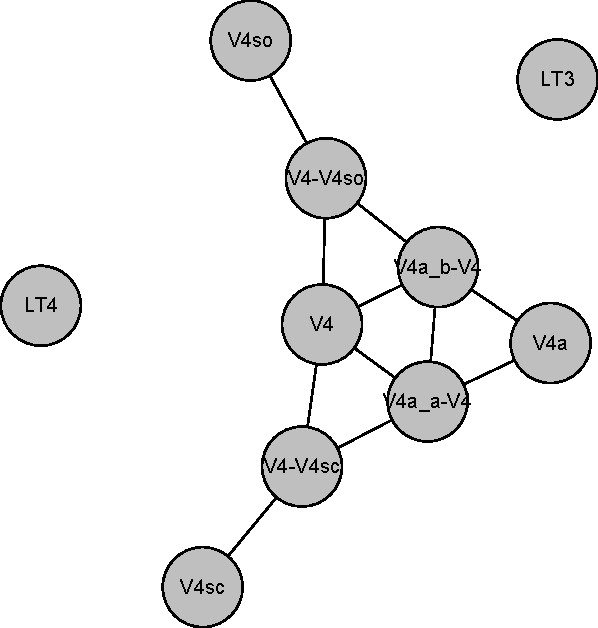
\includegraphics[scale=0.7]{id_example.pdf}
	\caption{Example of Inference Diagram}
	\label{fig:id_example}
\end{figure}



\section{Algorithms for diagnosability verification with virtual modules}
\label{sec:algorithms}

Assume that a language with a faulty behaviour and a language which has an
observable support are given. Then, it's required to verify if the observable
support is either for the faulty or non-faulty sublanguages. If it is true, then the
corresponding modules can be composed into a virtual module.
According to the Lemma \ref{lem:virtual_module_is_diagnosable}, in order to
decide if the virtual module is diagnosable we need to verify the necessary
conditions for all the strings $P_i^{-1}(L_{i,f})$ and $P_i^{-1}(L_{i,nf})$,
projected to the local languages of other modules $\{j \in I\mid j \neq i\}$.
Those local projections are the basic elements our algorithms operate with. In the sequel we
refer to the corresponding local sublanguages as to \emph{co-faulty} and
\emph{co-non-faulty} ones. A formal definition of these sublanguages is
presented below, and then an algorithm which computes the co-faulty
and co-non-faulty sublanguages for all the system's modules, is given. 
% It is
% followed by algorithms which verify diagnosability and find a virtual module.

\subsection{Co-faulty and co-non-faulty sublanguages}

\begin{definition}
\label{def:co-faulty}
Given $i, j \in I$, $L_{i,f} \subseteq L_i$,
we say that a sublanguage $L_{j,cf} \subseteq L_j$ is \emph{co-faulty} with
respect to $L_{i,f}$ if 
$$
	(\forall s \in L_{j,cf})(\forall t \in P_i[P_j^{-1}(s)])
	\left[
		t \in L_{i,f} \land t \not \in L_{i,nf}   
	\right],
$$ 
and a sublanguage $L_{j,cnf} \subseteq L_j$ is
\emph{co-non-faulty} with respect to $L_{i,nf}$ if 
$$
	(\forall s \in L_{j,cnf})(\forall t \in P_i[P_j^{-1}(s)])
	\left[
		t \not \in L_{i,f} \land t \in L_{i,nf}   
	\right].
$$ 
\end{definition}

In words, the co-faulty sublanguage is a sublanguage which satisfies two
conditions:
a) it is the sublanguage of projection of the global faulty language
to the local language; b) the sublanguage is not co-non-faulty.
Similarly, the co-non-faulty sublanguage is a sublanguage which satisfies
conditions:
a) it is the sublanguage of projection of the global non-faulty language
to the local language; b) the sublanguage is not co-faulty.

% \begin{lemma}
% \label{lem:empty_co_if_no_common}  
% Given a language $L_j\mid j \in I$, its co-faulty and
% co-non-faulty sublanguages are empty, if the language has no common events in
% its strings, i.e
% $$P_{\Sigma_j \rightarrow \bigcap_{i\neq j}^I \Sigma_i}(L_i) = \emptyset.$$
% \end{lemma}
% We skip the proof due to its triviality. 

Given global faulty and non-faulty sublanguages, one can compute the local
co-faulty sublanguage, using the global language, as follows:
\begin{equation}
\label{eq:co-faulty_from_global}
	\begin{array}{l}
		L_{j,cf} := P_j(L_f) \backslash P_j(L_{nf}),\\ 
		L_{j,cnf} := P_j(L_{nf}) \backslash P_j(L_{f}).	
	\end{array}
\end{equation}
However, we are interested to compute local sub languages without computing the
global language. Since the global faulty sublanguage is define as
\begin{equation}
\label{eq:co-faulty_from_locals}
	L_f := P_i^{-1}(L_{i,f}) \cap \bigcap_{k\neq
	i}^I P_k^{-1}(L_k),
\end{equation}
then, by substituting the global language in \ref{eq:co-faulty_from_global} by
\ref{eq:co-faulty_from_locals}, and by mathematical induction, the co-faulty
sublanguage of an arbitrary module can be computed as follows:

\begin{equation}
\label{eq:co-faulty_iterative_w_faulty}
	\begin{array}{l}
		L_{j,cf} := 
		\\
		P_j\Big(P_j^{-1}(L_j) \cap P_i^{-1}(L_{i,f})\cap 
		\bigcap_k^I P_k^{-1}(L_{k,cf})\Big) \backslash 
		\\
		P_j\Big(P_j^{-1}(L_j) \cap P_i^{-1}(L_{i,nf})\cap 
		\bigcap_k^I P_k^{-1}(L_{k,cnf})\Big),
		\\ 
		\textrm{where } i\neq j\neq k \in I.
	\end{array}
\end{equation}

We skip the definition of co-non-faulty sublanguage here due to its similarity. 


\subsection{Fault propagation algorithm}

\begin{alg}[!ht]
\caption{Forward propagation of a fault. Computes co-faulty and
co-non-faulty languages of all the modules}
\begin{algorithmic}[1]
	\Require The set of the system's languages $\{L_j\mid j \in I\}$, faulty and
	non-faulty sublanguages $L_{i,f}$, $L_{i,nf}$ of a faulty module $i\in I$.
	\ForAll{$j \in I$}
	\label{alg:fcf_init}
		\Comment{Initialization}
		\State $\Sigma_{j,c} \leftarrow \Sigma_j \cap \bigcup_{i\neq j}^I\Sigma_i$
		\State $C_j \leftarrow P_{j,c}(L_j)$
		\State $F_j \leftarrow \emptyset, N_j \leftarrow \emptyset$
	\EndFor
	\Procedure{propagate-fn}{$k$, $F_k$, $N_k$}
		\ForAll{$j \in I \mid j\neq k, \Sigma_j \cap \Sigma_k \neq \emptyset,
				\Sigma_{j,c}\neq \emptyset$} 
			\State $F'_j \leftarrow P_{j,c}(F_k \parallel C_j)$
			\label{alg:fcf_partial_begin}
			\State $N'_j \leftarrow P_{j,c}(N_k \parallel C_j)$ 
			\State $K \leftarrow \overline{F'_j \cap N'_j}$
			\State $F'_j \leftarrow F'_j \backslash K$
			\State $N'_j \leftarrow N'_j \backslash K$
			\label{alg:fcf_partial_end}
			\If{$F'_j \backslash F_j \neq \emptyset \lor 
				 N'_j \backslash N_j \neq \emptyset$}
				\label{alg:fcf_update}
				\State $F_j \leftarrow F_j \cup F'_j$
				\State $N_j \leftarrow N_j \cup N'_j$
				\State $\Sigma_{j,c} \leftarrow
					\{\sigma \in s \}$, where
				\State $s \in
						\left[(\overline{F_j} \backslash F_j) \cup
						(\overline{N_j} \backslash N_j)\right] \backslash	
						(\overline{F_j} \cap \overline{N_j})
						$
				\State \textproc{propagate-fn}$(j, F_j, N_j)$
			\EndIf
		\EndFor
	\EndProcedure
	
	\State $F_i \leftarrow P_{i,c}(L_{i,f})$
		\label{alg:fcf_Fi}
	\State $N_i \leftarrow P_{i,c}(L_{i,nf})$
	\State \textproc{propagate-fn}($i$, $F_i$, $N_i$)
	\Comment{Beginning of recursion}	
	\ForAll{$j \in I \mid j \neq i$}
		\Comment{Finalization}
		\label{alg:fcf_final}
		\State $L_{j,cf} \leftarrow L_j \cap P_{j,c}^{-1}(F_j)$
		\State $L_{j,cnf} \leftarrow L_j \cap P_{j,c}^{-1}(N_j)$
	\EndFor
	\\
	\Return $\{L_{j,cf}\}$, $\{L_{j,cnf}\}$
\end{algorithmic}
\label{alg:propagate_fn}
\end{alg}


Now, we present Algorithm \ref{alg:propagate_fn} which, given a module with a
faulty behaviour defined, computes the co-faulty and co-non-faulty languages for
all the rest modules of the system.
The algorithm starts from a preliminary step at line \ref{alg:fcf_init}.
At this step a projection to the common events $C_j$ is computed for all the
local languages. Projections of co-faulty and co-non-faulty sublanguages to the
common events, denoted as $F_j, N_j$, are empty in the beginning. Event sets
$\Sigma_{j,c}$ are sets of the common events, which don't belong neither to
co-faulty and co-non-faulty sublanguages nor to intersection of the
sublanguages' prefix-closures. Since that sublanguages are not defined in the
beginning, the event sets contain all events from the projections. A role of
these sets will be clarified later.
The recursive procedure \emph{propagate-fn} computes $F_j$ and $N_j$ for all the
system's modules, except the module with a fault; the procedure operates with
common events only. Before entering the procedure the projections of the faulty
module's sublanguages, $F_i, N_i$ are computed at the step \ref{alg:fcf_Fi}.
Note, that projection operation preserves faulty and non-faulty information,
when faulty behaviour is defined in a specification-based way.

The recursive procedure computes all projections $F_j, N_j$ of the modules
adjacent to a given module $k$ (we say that two modules are adjacent to each
other if their languages have events in common). At the first steps
\ref{alg:fcf_partial_begin}-\ref{alg:fcf_partial_end} of the procedure we
compute $F'_j, N'_j$ with respect to the module $k$; these projections are
partial. The parallel composition $F_k \parallel C_j$, followed by projection to
the common events, is used to extract the faulty information from the
language $F_k$ to $C_j$, and non-faulty from $N_k$ to $C_j$. At the step
\ref{alg:fcf_update} we check if some co-faulty or co-non-faulty strings should be added to the projections computed earlier. If so, then we update $F_j, N_j$, $\Sigma_{j,c}$ and call the same procedure to update projections of the adjacent modules. Thus, whenever the co-faulty or
co-non-faulty projections of that module changed, the projections $F_j, N_j$ are
updating with respect to every other module, due to recursion. The event sets
$\Sigma_{j,c}$ represent a potentiality that the projections $F_j, N_j$ can be
changed; the modules which have these sets empty can't change their language's
property with respect to the fault and, thus, are skipped during recursive
procedure. Finally, all the co-faulty and co-non-faulty sublanguages are
calculated for each module at the step \ref{alg:fcf_final}.



%%%%%%%%%%%%%%%%%%%%%%%%%%%%%%%%%%%%%%%%%%%%%%%%%%%%%%%%%%%%%%%%%%%%%%%%%%%%%%%
\subsection{Observation propagation algorithm}

\begin{alg} 
\caption{Backward propagation of the fault observation. Computes observable
information for the faulty module} 
\begin{algorithmic}[1]
	\Require The index  $i \in I$ of the faulty module, the index of a module with
	observable support $k \in I \mid M(L_{k,cf}) \neq \emptyset \lor M(L_{k,cnf})
	\neq \emptyset, k \neq i$, the sets $\{L_{j,cf}\}, \{L_{j,cnf}\}, j \in I$.
% 	\State $V \leftarrow \{i\}$ \Comment{Virtual module}

	\ForAll{$j \in I$}
	\label{alg:fco_init}
		\State $D_{j,f} \leftarrow P_{j,co}(L_{j,f})$
		\State $D_{j,nf} \leftarrow P_{j,co}(L_{j,nf})$
	\EndFor
	
	\Procedure{propagate-d}{$k$, $D_{k,f}$, $D_{k,nf}$}
		\ForAll{$j \in I \mid \Sigma_j \cap \Sigma_k \neq \emptyset$}
			\State $D'_{j,f} \leftarrow 
			P_{j,co}(F_j \parallel D_{k,f})$
			\If{$(D'_{j,f}\backslash D_{j,f} \neq \emptyset) \lor
				(D'_{j,nf}\backslash D_{j,nf} \neq \emptyset)$}
				\State $D_{j,f}\leftarrow D'_{j,f}$
				\State $D_{j,nf}\leftarrow D'_{j,nf}$
				\State \textproc{propagate-d}($j$, $D_{j,f}$, $D_{j,nf}$)
			\EndIf
		\EndFor 
	\EndProcedure
	
	\State \textproc{propagate-d}($k$, $D_{k,f}$, $D_{k,nf}$)
	\label{alg:fco_enter_recursion}
	\State $L_{i,f}^{ext} \leftarrow P_{i,co}(L_{i,f} \parallel D_{i,f})$
	\label{alg:fco_finalize}
	\State $L_{i,nf}^{ext} \leftarrow P_{i,co}(L_{i,nf} \parallel D_{i,nf})$
	\\
	\Return $L_{i,f}^{ext}, L_{i,nf}^{ext}$
\end{algorithmic}
\label{alg:propagate-d}
\end{alg}

The structure of the Algorithm \ref{alg:propagate-d} is similar to one
in Algorithm \ref{alg:propagate_fn}. It starts from computing projections to
common and observable events for the co-faulty and co-non-faulty sublanguages of each
module's language. Then, starting from the module $k$ which has observable
events in its sublanguages (i.e. it has potential observable support for a
sublanguage of the faulty module), begins a recursive procedure at step
\ref{alg:fco_enter_recursion}.
In the procedure we collect only observable events of other modules which are related to co-faulty or co-non-faulty
sublanguages. Then we propagated these events down to the faulty module.
Finally, at the step \ref{alg:fco_finalize}, the faulty and non-faulty
sublanguages of the faulty module are extended with observable events.

The result of the Algorithm \ref{alg:propagate-d}, the faulty and non-faulty
sublanguages extended with observable events, can be used to verify
diagnosability now. Any approach, which allows us to check for the presence of
indistinguishable strings in the language (the faulty and non-faulty
sublanguages can be united, if necessary), is suitable. We can have the
following outcomes after verification: a) no indistinguishable strings are
broken, b) no indistinguishable strings left, and c) some indistinguishable
strings are broken. In case (a) we pick another module $k \in I$ satisfying
requirements of the Algorithm \ref{alg:propagate-d} for further processing and
verification. In case (b) we may construct a virtual module of the faulty module
$i$ and the module $k$ and declare that the fault is diagnosable with respect to
the virtual module $\{i, k\}$ and stop, or continue and check if it exists
another module which can also be used to build a virtual module. In case (c) we should
pick additional module satisfying requirements of the Algorithm
\ref{alg:propagate-d} and continue the process until all the indistinguishable
strings are broken. The following section analyzes what may be considered as a
criteria for choosing the module with observable support $k$.


\subsection{Algorithm to choose a module with observable support}
Assume that the objective function is to have the number of modules in the
system as many as possible, i.e. to have the maximal cardinality of the
partition $J$.
Given an initial set of languages, let rank of $J$ be equal to 0, i.e. $|J| =
|I|$. Let $F$ denotes the subset of languages with faults, and $M$ denotes the
subset of languages with corresponding observable supports.
Assume that it is always possible to make the system modularly diagnosable with
respect to some virtual modules. Then we know that $(\forall f \in F)~\exists m
\in M$. Let $F \cap M = \emptyset$ and $|M| \geq |F|$. Then, to make the system
modularly diagnosable it is required, in the worst case, $|F|$ members of $M$.
Thus, the cardinality of the systems with virtual modules, i.e. the cardinality
of the partition, in the worst case is:
\begin{equation}
	\min |J| = |I| - |F|.
\end{equation}
Let $M \subseteq F$. Then, the cardinality of the partition in the best case
is:
\begin{equation}
	\max |J| = |I| - \left(
		\left\lfloor \frac{|F|}{2} \right\rfloor + \textrm{mod} \frac{|F|}{2}
		\right). 
\end{equation}

As can be seen from the above, in order to maximize the number of modules while
making the virtual modules, we should consider, firstly, the modules which
themselves have faults. We propose a procedure for the given objective function
as follows:

Given the system of cardinality $|I|$, the subset $F \subseteq I$ of modules
with faults, such that any $f\in F$ is not diagnosable locally, the subset $M
\subseteq I$ of modules with observable supports, such that $(\forall f \in
F)~\{m \in M\}\neq \emptyset$. In order to make the system diagnosable by
the minimal number of virtual modules:
\begin{enumerate}
  \item Initially set the partition $J$ of $I$ such that the rank of $J$ is
  equal to 0;
  \item $(\forall j \in J, f \in j)$ update $j$ as follows: 
  	$j := j \cup \{m \in M \cap F\}$ if $M \cap F \neq \emptyset$,
 $j := j \cup \{m \in M\}$ otherwise, where $\{m\}$ is a singleton of the
 arbitrary chosen observable support for the given $f$, such that the new $j$
 is locally diagnosable; exclude $m$ from $k \in J \mid k \neq j$, and remove
 $k$ from $J$ if $k=\emptyset$.
\end{enumerate} 
The order the observable supports are verified in the procedure guaranties that
we consider the languages which themselves contain the faulty
sublanguages at first, thus maximizing the number of virtual modules in the
system.

It worth to note that the above algorithm can be augmented by additional
criteria aimed, for instance, to decrease computational burden.


%%%%%%%%%%%%%%%%%%%%%%%%%%%%%%%%%%%%%%%%%%%%%%%%%%%%%%%%%%%%%%%%%%%%%%%%%%%%%%%
\section{Example}
\label{sec:Example}
An example with languages presented by automata (see the Figures \ref{fig:G1-4}
-- \ref{fig:L1_extended}) shows how the algorithms \ref{alg:propagate_fn} and
\ref{alg:propagate-d} can be applied to a simple system. We use marked states to
mark strings in languages, since they are not prefix-closed, in general. The
system consists of three modules as depicted in Figure \ref{fig:G1-4}. Here a
fault is presented only in the language $L_1$ by the event $f$.
Figure \ref{fig:G1_faulty} depicts faulty and non-faulty sublanguages of the
language $L_1$. Projections of these sublanguages to the common events (step
\ref{alg:fcf_Fi} of the Algorithm \ref{alg:propagate_fn}), $F_1$ and $N_1$ are
depicted in the Figure \ref{fig:FN}. Suppose that in the beginning of the
recursive procedure we pick module $2$. The figure depicts the co-faulty
and co-non-faulty sublanguage of the language $L_2$ with respect to the language
$L_1$, calculated at the steps \ref{alg:fcf_partial_begin} of the algorithm (we
don't show intermediate automata, reflecting compositional steps, due to space
restrictions). Note, that, when calculated, the event set $\Sigma_{2,c}$ is
empty for module $2$. Hence this module will not participate in the procedure
as a module adjacent to others. At the next step we randomly pick the language
$L_4$, and compute $F_4$ and $N_4$ with respect to the module $2$. Now, note
that $\Sigma_{3,c}:= \{e\}$, since this event is neither in the co-faulty and
co-non-faulty projections nor in their common prefix. The iterations is followed
by the module $3$, which has module $4$ as an adjacent one. Therefore, the
sublanguages of this module are updated.

Figure \ref{fig:L4_f} depicts co-faulty and co-non-faulty sublanguages of module
$4$ calculated at the step \ref{alg:fco_finalize} of the Algorithm
\ref{alg:propagate_fn}. It shows that the co-faulty sublanguage of the module
has an observable support; it satisfies the requirements of the Lemma
\ref{lem:distinguished}. Other modules with no faults have no observable
events; they have no observable supports, and not depicted.

The major steps of Algorithm \ref{alg:propagate-d} are depicted in the Figure
\ref{fig:D}. It is shown how the observable information from the module $4$ is
propagated backward to the language of the module $1$. The final step of the
algorithm is depicted in the Figure \ref{fig:L1_extended}. Clearly, the faulty
and non-faulty sublanguages, extended with observable information, have
distinguished observations. Then, we can conclude that the virtual module
composed of the modules $1$ and $4$ is locally diagnosable. Hence, the system is
modularly diagnosable with modularity presented by the partition 
$\{\{1,4\}, \{2\}, \{3\}\}$.



\begin{figure}[t]
\centering
\begin{tikzpicture}[->,>=stealth, node distance=2cm, auto, shorten >=1pt,
semithick, initial text=,	
	every node/.style={scale=0.8},
    every state/.style={fill=green!40,text=black},
    accepting/.style={double distance=1.5pt, outer sep=0.75pt+\pgflinewidth}
    ]
% \draw[help lines] (0,-2) grid (6,2);
% G1
\node[initial,state] (0)                    {$0$};
\node[above left = 0.5em of 0]{$L_{1}$};
\node[state, accepting]         (1) [above right of=0] {$1$};
\node[state, accepting]         (2) [right of=1]       {$2$};
\node[state, accepting]         (3) [right of=2]       {$3$};
\node[state, accepting]         (4) [right of=3]       {$4$};
\node[state, accepting]         (5) [right of=0] 		{$5$};
\node[]         () [below right of=0] 		{}; %some blank space
\path
(0)	edge [] 		 node {$f$} (1)
(1)	edge [] 		 node {$a$} (2)
(2)	edge [] 		 node {$o_1$} (3)
(3)	edge [] 		 node {$b$} (4)
(4)	edge [loop right] node {$c$} (4)
(0)	edge [] 		 node {$o_1$} (5)
(5)	edge [loop right] node {$c$} (5)
;
\end{tikzpicture}
\begin{tikzpicture}[->,>=stealth, node distance=2cm, auto, shorten >=1pt,
semithick, initial text=,	
	every node/.style={scale=0.8},
    every state/.style={fill=green!40,text=black},
    accepting/.style={double distance=1.5pt, outer sep=0.75pt+\pgflinewidth}
    ]
% \draw[help lines] (0,-2) grid (6,2);
% G2
\node[initial,state, accepting] (0)                    {$0$};
\node[above left = 0.5em of 0]{$L_{2}$};
\node[state, accepting]         (1) [right of=0] 		{$1$};
\node[state, accepting]         (2) [right of=1]       {$2$};
\path
(0)	edge [] 		  node {$a$} (1)
	edge [loop below] node {$c$} (0)
(1)	edge [] 		  node {$d$} (2)
(2)	edge [loop right] node {$c$} (2)
;
\end{tikzpicture}
\begin{tikzpicture}[->,>=stealth, node distance=2cm, auto, shorten >=1pt,
semithick, initial text=,	
	every node/.style={scale=0.8},
    every state/.style={fill=green!40,text=black},
    accepting/.style={double distance=1.5pt, outer sep=0.75pt+\pgflinewidth}
    ]
% G3
% \node[initial,state, accepting] (0') [below of=0]      {$0$};
\node[initial,state, accepting] (0') []      {$0$};
\node[above left = 0.5em of 0']{$L_{3}$};
\node[state, accepting]         (1') [right of=0']		{$1$};
\node[state, accepting]         (2') [right of=1']     {$2$};
\path
(0')	edge [] 		  node {$b$} (1')
		edge [loop below] node {$c$} (0')
(1')	edge [] 		  node {$e$} (2')
(2')	edge [loop right] node {$c$} (2')
;
\end{tikzpicture}
\begin{tikzpicture}[->,>=stealth, node distance=2cm, auto, shorten >=1pt,
semithick, initial text=,	
	every node/.style={scale=0.8},
    every state/.style={fill=green!40,text=black},
    accepting/.style={double distance=1.5pt, outer sep=0.75pt+\pgflinewidth}
    ]
% G4
% \node[initial,state, accepting] (0'') [below of=0']  {$0$};
\node[initial,state, accepting] (0'') []  {$0$};
\node[] (fake) [above of=0''] {}; %for space above the picture
\node[above left = 0.5em of 0'']{$L_{4}$}; 
\node[state, accepting]         (1'') [right of=0'']	{$1$};
\node[state, accepting]         (2'') [right of=1'']   {$2$};
\node[state, accepting]         (3'') [right of=2'']   {$3$};
\path
(0'')	edge [] 		  node {$e$} (1'')
		edge [loop below] node {$c$} (0'')
(1'')	edge [] 		  node {$o_2$} (2'')
(2'')	edge [] 		  node {$d$} (3'')
(3'')	edge [loop right] node {$c$} (3'')
;
\end{tikzpicture}
\caption{Automata marking languages $L_1, L_2, L_3$ and $L_4$. $\Sigma_o :=
\{o_1, o_2\}$, $\Sigma_f := \{f\}$}
\label{fig:G1-4}
\end{figure}

% Fautly and non-faulty
\begin{figure}[t]
% \centering
\begin{tikzpicture}[->,>=stealth, node distance=2cm, auto, shorten >=1pt,
semithick, initial text=,	
	every node/.style={scale=0.8},
    every state/.style={fill=green!40,text=black},
    accepting/.style={double distance=1.5pt, outer sep=0.75pt+\pgflinewidth}
    ]
% \draw[help lines] (0,-2) grid (6,2);
\node[initial,state] (0)                    {$0$};
% \node[above = 3em of 0] {}; %adds some space above
\node[above left = 0.5em of 0]{$L_{1,f}$};
\node[state, accepting, fill=orange]         (1) [right of=0] 		{$1$};
\node[state, accepting, fill=orange]         (2) [right of=1]       {$2$};
\node[state, accepting, fill=orange]         (3) [right of=2]       {$3$};
\node[state, accepting, fill=orange]         (4) [right of=3]       {$4$};

\node[initial,state] (0') [below of=0]                   {$0$};
\node[above left = 0.5em of 0']{$L_{1,nf}$};
\node[state, accepting]         (5)
[right of=0'] 		{$5$};

\path
(0)	edge [] 		 node {$f$} (1)
(1)	edge [] 		 node {$a$} (2)
(2)	edge [] 		 node {$o_1$} (3)
(3)	edge [] 		 node {$b$} (4)
(4)	edge [loop below] node {$c$} (4)
;
\path
(0') edge [] 		 node {$o_1$} (5)
(5)	edge [loop right] node {$c$} (5)
;
\end{tikzpicture}
\caption{Automata marking the faulty and non-faulty sublanguages of $L_1$}
\label{fig:G1_faulty}
% \end{figure}

% Projection to common events (G1)
% \begin{figure}[t!]
% \centering
\begin{tikzpicture}[->,>=stealth, node distance=2cm, auto, shorten >=1pt,
semithick, initial text=,	
	every node/.style={scale=0.8},
    every state/.style={fill=green!40,text=black},
    accepting/.style={double distance=1.5pt, outer sep=0.75pt+\pgflinewidth}
    ]
% \draw[help lines] (0,-2) grid (6,2);
\node[initial,state] (0)                    {$0$};
% \node[above = 3em of 0] {}; %adds some space above
\node[above left = 0.5em of 0]{$F_1$};
\node[state, accepting, fill=orange]         (2) [right of=0]       {$2$};
\node[state, accepting, fill=orange]         (4) [right of=2]       {$4$};

\node[initial,state] (0') [] at (6,0)              {$0$};
\node[above left = 0.5em of 0']{$N_1$};
\node[state, accepting]         (5) [right of=0'] 		{$5$};

\path
(0)	edge [] 		 node {$a$} (2)
(2)	edge [] 		 node {$b$} (4)
(4)	edge [loop right] node {$c$} (4)
;
\path
(0') edge [] 		 node {$c$} (5)
(5)	edge [loop right] node {$c$} (5)
;
\end{tikzpicture}
\\

\begin{tikzpicture}[->,>=stealth, node distance=2cm, auto, shorten >=1pt,
semithick, initial text=,	
	every node/.style={scale=0.8},
    every state/.style={fill=green!40,text=black},
    accepting/.style={double distance=1.5pt, outer sep=0.75pt+\pgflinewidth}
    ]
% \draw[help lines] (0,-2) grid (6,2);
% F2
\node[initial,state] (0)                    {$0$};
\node[above left = 0.5em of 0]{$F_2$};
\node[state, accepting, fill=orange]         (1) [right of=0] 		{$1$};
\node[state, accepting, fill=orange]         (2) [right of=1]       {$2$};
\path
(0)	edge [] 		  node {$a$} (1)
(1)	edge [] 		  node {$d$} (2)
(2)	edge [loop right] node {$c$} (2)
;
% F2
\node[initial,state, accepting] (0') at (6,0) {$0$};
\node[above left = 0.5em of 0']{$N_2$};
\path
(0') edge [loop below] node {$c$} (0')
;
\end{tikzpicture}

\newline

\begin{tikzpicture}[->,>=stealth, node distance=2cm, auto, shorten >=1pt,
semithick, initial text=,	
	every node/.style={scale=0.8},
    every state/.style={fill=green!40,text=black},
    accepting/.style={double distance=1.5pt, outer sep=0.75pt+\pgflinewidth}
    ]
% \draw[help lines] (0,-2) grid (6,2);
% F4
\node[initial,state] (0)                    {$0$};
\node[above left = 0.5em of 0]{$F_4$};
\node[state ]         (1) [right of=0] 		{$1$};
\node[state, accepting, fill=orange]         (2) [right of=1]       {$2$};
\path
(0)	edge [] 		  node {$e$} (1)
(1)	edge [] 		  node {$d$} (2)
(2)	edge [loop right] node {$c$} (2)
;
\node[initial,state, accepting] (0') at (6,0) {$0$};
\node[above left = 0.5em of 0']{$N_4$};
\path
(0') edge [loop below] node {$c$} (0')
;
\end{tikzpicture}

\newline

\begin{tikzpicture}[->,>=stealth, node distance=2cm, auto, shorten >=1pt,
semithick, initial text=,	
	every node/.style={scale=0.8}, 
	every state/.style={fill=green!40,text=black},
    accepting/.style={double distance=1.5pt, outer sep=0.75pt+\pgflinewidth}
    ]
% \draw[help lines] (0,-2) grid (6,2);
% F3
\node[initial,state] (0)                    {$0$};
\node[above left = 0.5em of 0]{$F_3$};
\node[state, accepting, fill=orange]         (1) [right of=0] 		{$1$};
\node[state, accepting, fill=orange]         (2) [right of=1]       {$2$};
\path
(0)	edge [] 		  node {$b$} (1)
(1)	edge [] 		  node {$e$} (2)
(2)	edge [loop right] node {$c$} (2)
;
\node[initial,state, accepting] (0') at (6,0) {$0$};
\node[above left = 0.5em of 0']{$N_3$};
\path
(0') edge [loop below] node {$c$} (0')
;
\end{tikzpicture}

\newline

\begin{tikzpicture}[->,>=stealth, node distance=2cm, auto, shorten >=1pt,
semithick, initial text=,	
	every node/.style={scale=0.8},
    every state/.style={fill=green!40,text=black},
    accepting/.style={double distance=1.5pt, outer sep=0.75pt+\pgflinewidth}
    ]
% \draw[help lines] (0,-2) grid (6,2);
% F4
\node[initial,state] (0)                    {$0$};
\node[above left = 0.5em of 0]{$F_4$};
\node[state, accepting, fill=orange]         (1) [right of=0] 		{$1$};
\node[state, accepting, fill=orange]         (2) [right of=1]       {$2$};
\path
(0)	edge [] 		  node {$e$} (1)
(1)	edge [] 		  node {$d$} (2)
(2)	edge [loop right] node {$c$} (2)
;
\node[initial,state, accepting] (0') at (6,0) {$0$};
\node[above left = 0.5em of 0']{$N_4$};
\path
(0') edge [loop below] node {$c$} (0')
;
\end{tikzpicture}

\caption{Automata marking sublanguages $F_1$ and $N_1$ of the faulty module,
and co-faulty and co-non-faulty languages of the modules 2, 3 and 4 in the
order they are composed (top-down): 1-2, 2-4, 1-3, 3-4. Note, that the
sublanguage $F_4$ is defined partially at first, then fully}
\label{fig:FN}
\end{figure}

% Fautly and non-faulty
\begin{figure}[t]
% \centering
\begin{tikzpicture}[->,>=stealth, node distance=2cm, auto, shorten >=1pt,
semithick, initial text=,	
	every node/.style={scale=0.8},
    every state/.style={fill=green!40,text=black},
    accepting/.style={double distance=1.5pt, outer sep=0.75pt+\pgflinewidth}
    ]
\node[initial,state] (0) {$0$};
\node[above = 0.5em of 0]{$L_{4,cf}$}; 
\node[state, accepting, fill=orange]         (1) [right of=0]	{$1$};
\node[state, accepting, fill=orange]         (2) [right of=1]   {$2$};
\node[state, accepting, fill=orange]         (3) [right of=2]   {$3$};
\path
(0)	edge [] 		  node {$e$} (1)
(1)	edge [] 		  node {$o_2$} (2)
(2)	edge [] 		  node {$d$} (3)
(3)	edge [loop right] node {$c$} (3)
;
\node[initial,state, accepting] (0') [below of=0] {$0$};
\node[above left = 0.5em of 0']{$L_{4,cnf}$};
\path
(0') edge [loop below] node {$c$} (0')
;
\end{tikzpicture}
\caption{Automata marking co-faulty and co-non-faulty sublanguages of
the language $L_4$. Automata for the sublanguages of the modules 2 and 3 are
equal to the ones depicted in the Figure \ref{fig:FN}}
\label{fig:L4_f}
% \end{figure}

% Projections to common and observable events
% \begin{figure}[t]
\begin{tikzpicture}[->,>=stealth, node distance=2cm, auto, shorten >=1pt,
semithick, initial text=,	
	every node/.style={scale=0.8}, 
	every state/.style={fill=green!40,text=black},
    accepting/.style={double distance=1.5pt, outer sep=0.75pt+\pgflinewidth}
    ]
% \draw[help lines] (0,-2) grid (6,2);
% F3
\node[initial,state] (0)                    {$0$};
% \node[above = 3em of 0] {}; %adds some space above
\node[above left = 0.5em of 0]{$D_{3,f}$};
\node[state, accepting, fill=orange]         (1) [right of=0] 		{$1$};
\node[state, accepting, fill=orange]         (2) [right of=1]       {$2$};
\node[state, accepting, fill=orange]         (2') [right of=2]       {$2'$};
\path
(0)	edge [] 		  node {$b$} (1)
(1)	edge [] 		  node {$e$} (2)
(2)	edge [] 		  node {$o_2$} (2')
(2')	edge [loop right] node {$c$} (2')
;
\end{tikzpicture}
\begin{tikzpicture}[->,>=stealth, node distance=2cm, auto, shorten >=1pt,
semithick, initial text=,	
	every node/.style={scale=0.8},
    every state/.style={fill=green!40,text=black},
    accepting/.style={double distance=1.5pt, outer sep=0.75pt+\pgflinewidth}
    ]
\node[initial,state] (0)                    {$0$};
\node[above left = 0.5em of 0]{$D_{2,f}$};
\node[state, accepting, fill=orange]         (1) [right of=0] 		{$1$};
\node[state, accepting, fill=orange]         (1') [right of=1] 		{$1'$};
\node[state, accepting, fill=orange]         (2) [right of=1']       {$2$};
\path
(0)	edge [] 		  node {$a$} (1)
(1)	edge [] 		  node {$o_2$} (1')
(1')edge [] 		  node {$d$} (2)
(2)	edge [loop right] node {$c$} (2)
;
\end{tikzpicture}
\begin{tikzpicture}[->,>=stealth, node distance=2cm, auto, shorten >=1pt,
semithick, initial text=,	
	every node/.style={scale=0.8},
    every state/.style={fill=green!40,text=black},
    accepting/.style={double distance=1.5pt, outer sep=0.75pt+\pgflinewidth}
    ]
% \draw[help lines] (0,-2) grid (6,2);
\node[initial,state] (0)                    {$0$};
\node[above left = 0.5em of 0]{$D_{1,f}$};
\node[state, accepting, fill=orange]         (2) [right of=0]       {$2$};
\node[state, accepting, fill=orange]         (2') [below of=2]      
{$2'$}; \node[state, accepting, fill=orange]         (4) [right of=2]      {$4$};
\node[state, accepting, fill=orange]         (4')[below of=4]{$4'$};
\path
(0)	edge [] 		 node {$a$} (2)
(2)	edge [] 		 node {$b$} (4)
	edge [] 		node {$o_2$} (2')
(2')edge [] 		 node {$b$} (4')
(4)	edge [loop right] node {$c$} (4)
	edge [] 		node {$o_2$} (4')
(4')edge [loop right] node {$c$} (4')
;
\end{tikzpicture}
\begin{tikzpicture}[->,>=stealth, node distance=2cm, auto, shorten >=1pt,
semithick, initial text=,	
	every node/.style={scale=0.8},
    every state/.style={fill=green!40,text=black},
    accepting/.style={double distance=1.5pt, outer sep=0.75pt+\pgflinewidth}
    ]
% \draw[help lines] (0,-2) grid (6,2);
\node[initial,state] (0)                    {$0$};
\node[above left = 0.5em of 0]{$D_{1,f}$};
\node[state, accepting, fill=orange]         (2) [right of=0]       {$2$};
\node[state, accepting, fill=orange]         (4) [right of=2]       {$4$};
\node[state, accepting, fill=orange]         (4')[right of=4] {$4'$};
\path
(0)	edge [] 		 node {$a$} (2)
(2)	edge [] 		 node {$b$} (4)
(4) edge [] 		node {$o_2$} (4')
(4')edge [loop right] node {$c$} (4')
;
\end{tikzpicture}
\caption{Automata marking $D_{j,f}$ of the modules 1, 2 and 3 in
the order they are composed (top-down): 4-3, 4-2, 2-1, 3-1. Automata marking
$D_{j,nf}$ are not depicted since they have no observable events}
\label{fig:D}
% \end{figure}


% Fautly and non-faulty
% \begin{figure}[t!]
% \centering
\begin{tikzpicture}[->,>=stealth, node distance=2cm, auto, shorten >=1pt,
semithick, initial text=,	
	every node/.style={scale=0.8},
    every state/.style={fill=green!40,text=black},
    accepting/.style={double distance=1.5pt, outer sep=0.75pt+\pgflinewidth}
    ]
% \draw[help lines] (0,-2) grid (6,2);
\node[initial,state] (0)                    {$0$};
% \node[above = 3em of 0] {}; %adds some space above
\node[above left = 0.5em of 0]{$L_{1,f}$};
\node[state, accepting, fill=orange]         (1) [right of=0] 		{$1$};
\node[state, accepting, fill=orange]         (2) [right of=1]       {$2$};
\node[state, accepting, fill=orange]         (3) [right of=2]       {$3$};
\node[state, accepting, fill=orange]         (4) [right of=3]       {$4$};
\node[state, accepting, fill=orange]         (4')[right of=4]       {$4'$};

\node[initial,state] (0') [below of=0]                   {$0$};
\node[above left = 0.5em of 0']{$L_{1,nf}$};
\node[state, accepting]         (5)
[right of=0'] 		{$5$};

\path
(0)	edge [] 		 node {$f$} (1)
(1)	edge [] 		 node {$a$} (2)
(2)	edge [] 		 node {$o_1$} (3)
(3)	edge [] 		 node {$b$} (4)
(4) edge [] 		 node {$o_2$} (4')
(4')edge [loop below] node {$c$} (4')

;
\path
(0') edge [] 		 node {$o_1$} (5)
(5)	edge [loop right] node {$c$} (5)
;
\end{tikzpicture}
\caption{Automata marking the faulty and non-faulty sublanguages of $L_1$ after
the backward Algorithm. The observation of $L_{1,f}$ is $\{o_1o_2\}$ differs
from the observation of $L_{1,nf}$ which is $\{o_1\}$}
\label{fig:L1_extended}
\end{figure}


\section{Related approaches}

The notion of virtual modular diagnosability was initially introduced in this
work. However, this approach can be decomposed into a few techniques, and a
few works, each solving similar problems, can be found in literature. These
studies are described in the following.

An interesting approach is developed in \cite{rudie_minimal_1999},
\cite{rudie_minimal_2003} and \cite{lin_minimal_2007} where the authors start
from the assumption that the modules of a system require communication to each
other in order to make a decision (e.g. about a failure), but the information
they exchange can be redundant. They try to minimize communications globally and
provide a solution with exponential time complexity. This approach is
completely different to the one presented in this work, since it does not change
modularity of the system. However, the idea to reduce redundant communication
may result in a higher modularity in our context.

In \cite{ye_incremental_2009} and \cite{ye_general_2012} the authors verify
distributed diagnosability where the failures are presented as ``patterns'',
i.e. as sequences of events, rather then singular fault events. 
The modularity of the system doesn't change, however there some similarities
in the failure modeling and the algorithms. The notion
of patterns in that work can be seen equal to the specification-based (or
state-based) failure representation in our work. The diagnosability property is
verified incrementally, without construction of the global language. The authors
use reduction of the languages with respect to observable and common events, but
do it simultaneously. Their algorithms differ from the algorithms in our
approach, since here the forward-back two way propagation computation is used in
order to reduce space complexity even more.

The work \cite{fabre_partial_2007} describes partial order techniques for
distributed event systems and underlines their importance for solving
a variety of problems without computing global language of a system. The
authors use notion of ``interaction graph" similar to the notion of ``inference
diagram'' and explore it in a similar manner, but they do not address problems
of diagnosability verification.  
 
A work presented in \cite{su_global_2005} is also similar in terms of the
algorithm. The authors introduce notion of \emph{global consistency}, which
assumes that observable projection of each module's language accounts all the
interaction with other languages of the system, i.e. a sublanguage 
$L'_i \subseteq M_i(L_i)$ is globally consistent if 
$L'_i = M_i(\parallel_j(M_j(L_j)))$, where $i, j \in I$. After achieving global
consistency the local diagnosers are computed, and a global decision on a
failure occurrence is performed based on decisions of each diagnoser. The
algorithm for computation of globally consistent projections differs from ours
since it defines all the observable information firstly, and only then
applies a knowledge about failures. In our algorithm the failure information is
propagated firstly with no space growth. Then the backward propagation algorithm
collects an observable information only for indistinguishable strings. Thus, the
state complexity of our approach may be lower. However, all the advantages of
the authors' approach, such the heuristic node selection procedure, can applied
for our approach too.

In \cite{pencole_diagnosability_2004} the authors present the approach which is
the closest to the our, since they introduce a notion of \emph{subsystem}, which
is equal to the notion of virtual module in a sense that a failure originated
from one module of the subsystem is diagnosable using observations of the
modules of the same subsystem. The algorithms are different. Beside this, our
work arguments the aforementioned approach with inference diagram exploration,
sufficient and necessary conditions for diagnosability (i.e.
diagnosability-related structural patterns) and the heuristic procedure for
the creation of the locally diagnosable subsystems.
